% ITEX root = ../Campos_Matthew_CMEE_2020.tex
\subsection{Cauchy Distribution}
\begin{wrapfigure}{r} {0.7\textwidth}
    \begin{center}
        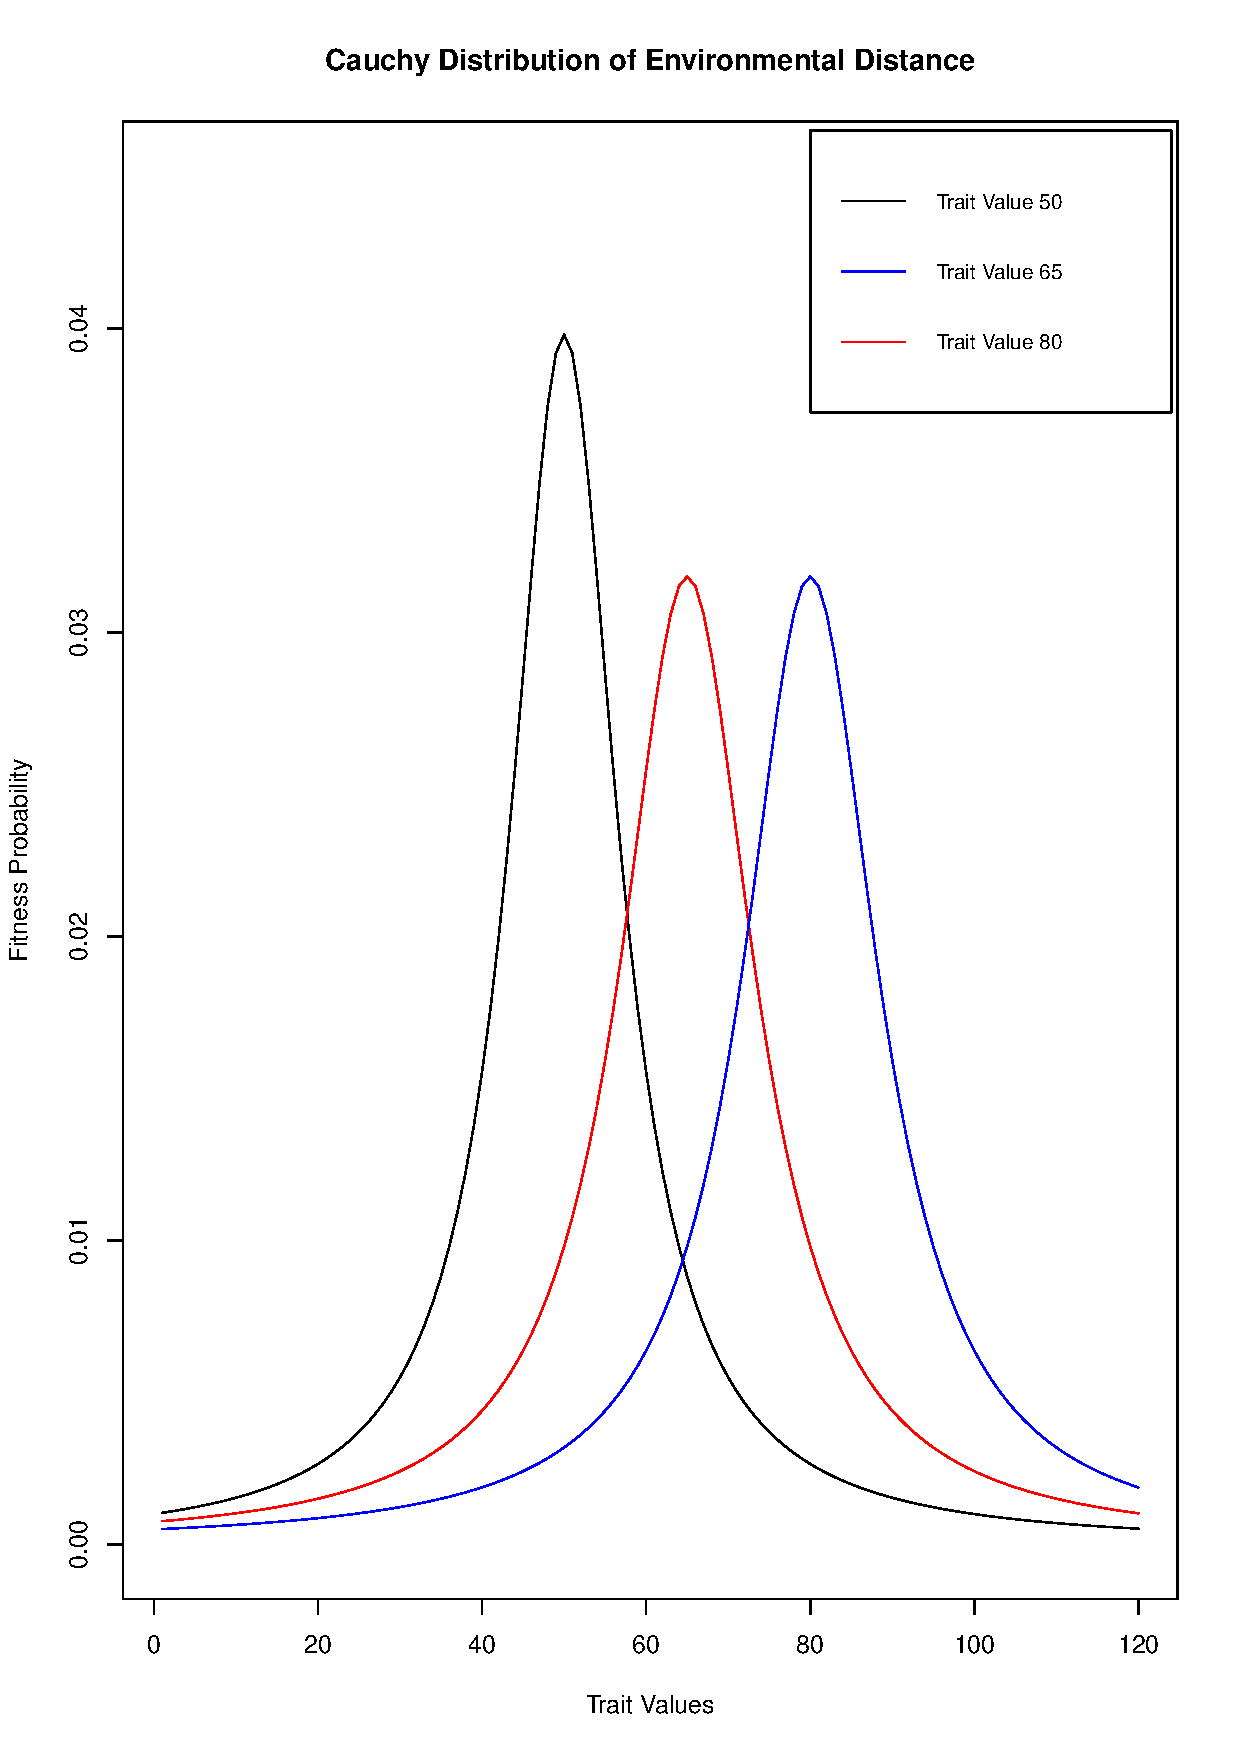
\includegraphics[scale=0.2]{../Results/Cauchy_Distribution.pdf}
    \end{center}
    \caption{Plot of the Cauchy Distribution used to derive fitness probabilities (for reproduction) and fitness values (normalising) of individuals. Distribution is also representative of the environmental distances respective populations evolved to. The main population (black) evolved to a trait value of 50, where the peak trait value has a reproductive probability of 3.98\%. Migrant populations either evolved to a trait value of 65 (blue) or 80 (red).}
    \label{fig:Cauchy Distribution}
\end{wrapfigure}
A Cauchy distribution was used to determine the fitness values based on trait values. The plot on the right shows how the shape of the distribution is similar to a normal distribution as seen in \textit{figure 2}. The peak represents the median, in this case the maximum probability a trait has of passing on to the next generation. Unlike a normal distribution, it is narrower within the curve. Even with large standard deviation, \textit{figure 2} shows how small deviations from the desired trait values can significant decline in probability of an individual being selected for reproduction. These desired trait values represent the environment and the distance between them is the \textit{environmental distance}. Individuals within their populations are evolving to their respective peaks. Long tail distribution allowed for the possibility of migrant genes values persisting for generations, allowing investigation into how the network develops with invading alleles.
\subsection{No Migration}
\begin{figure}[h]
    \centering
        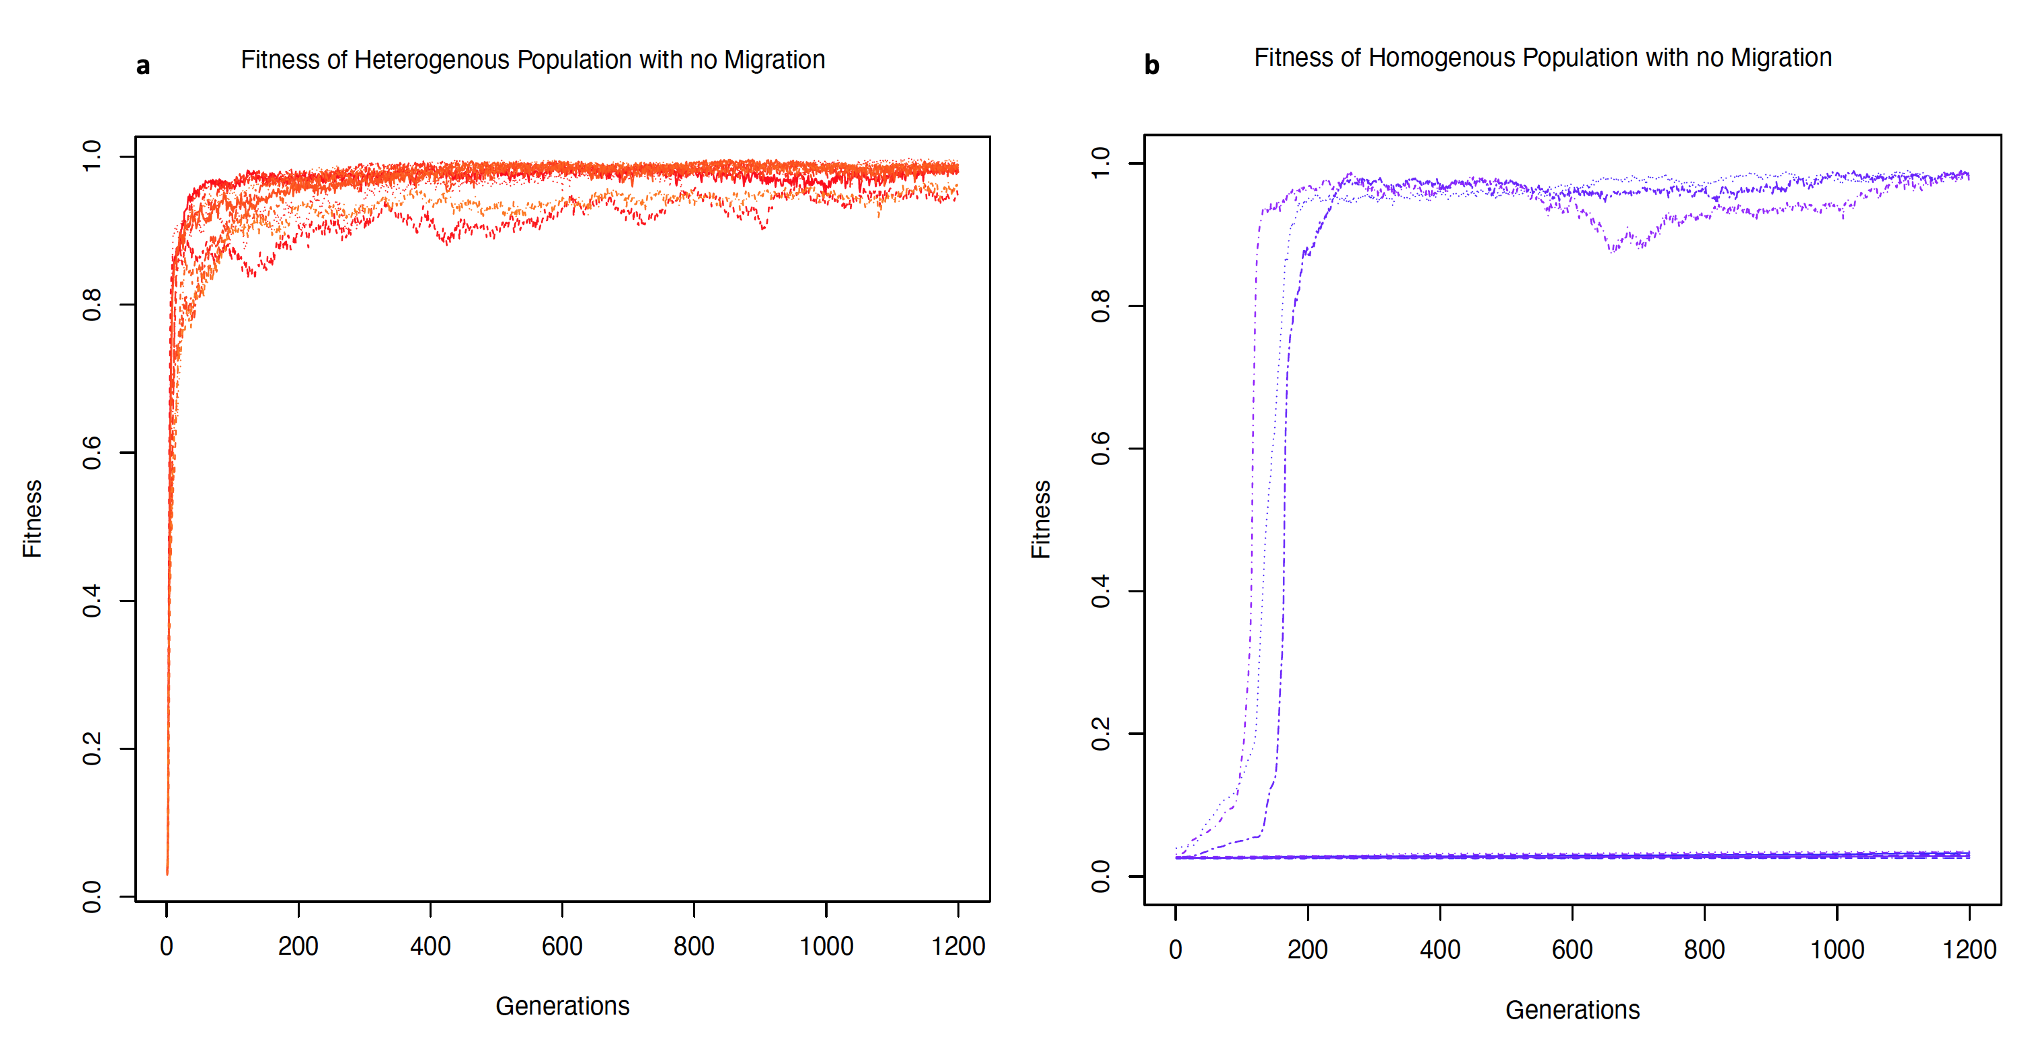
\includegraphics[scale=0.3]{../Results/early_no_migration.jpg}
    \caption{graphs showing the fitness evolution without migration for the populations that started as heterozygous or homozygous. (a) shows the evolution of a network that is homogenous network, where all starting allele values are the same per site per individual, randomly generated using a uniform distribution between 0.10 and 0.30. (b) shows how a heterogenous network evolves where starting values (between 0.10 and 0.30) for each site are different. Homogenous populations rarely evolved and had a mean fitness of 0.165, standard deviation of 0.035 while the heterogenous populations had an average fitness value of 0.955 with a standard deviation of 0.324.}
    \label{fig:No Migration}
\end{figure}
\textit{Figure 3} plots the fitness values of starting homogenous and heterogenous population, they both show rapid evolution and have very similar patterns of sharp gradients in the early generations. The graphs shows how genetic variation helps a population evolve rapidly while homogenous rely on chance beneficial scenarios to improve fitness. A population that began as heterogenous evolves faster as there was greater variation in the allele values, allowing for better combinations to be selected for. Gradients of the line at the start are steep and vary once it begins to plateau.\\
The results show that when there is no migration happening, the genetic network does evolve rapidly to the desired trait values. In a very short time period, it reaches an average fitness of 0.955. Normalising the fitness reveals how rapidly the trait values rises to 50, plateauing around a fitness value of 1 well within 100 generations. Although there are cases of the fitness deviating, overall the rise to the average fitness is steep. The homozygous population had a lot more noise throughout the simulation. There were instances where the population did not even increase in fitness and stayed near within the confine of its starting fitness value. There are a few instances where fitness sharply rose to around 1.00 and stayed there.
\subsection{Migration}
\begin{figure}[h]
    \centering
        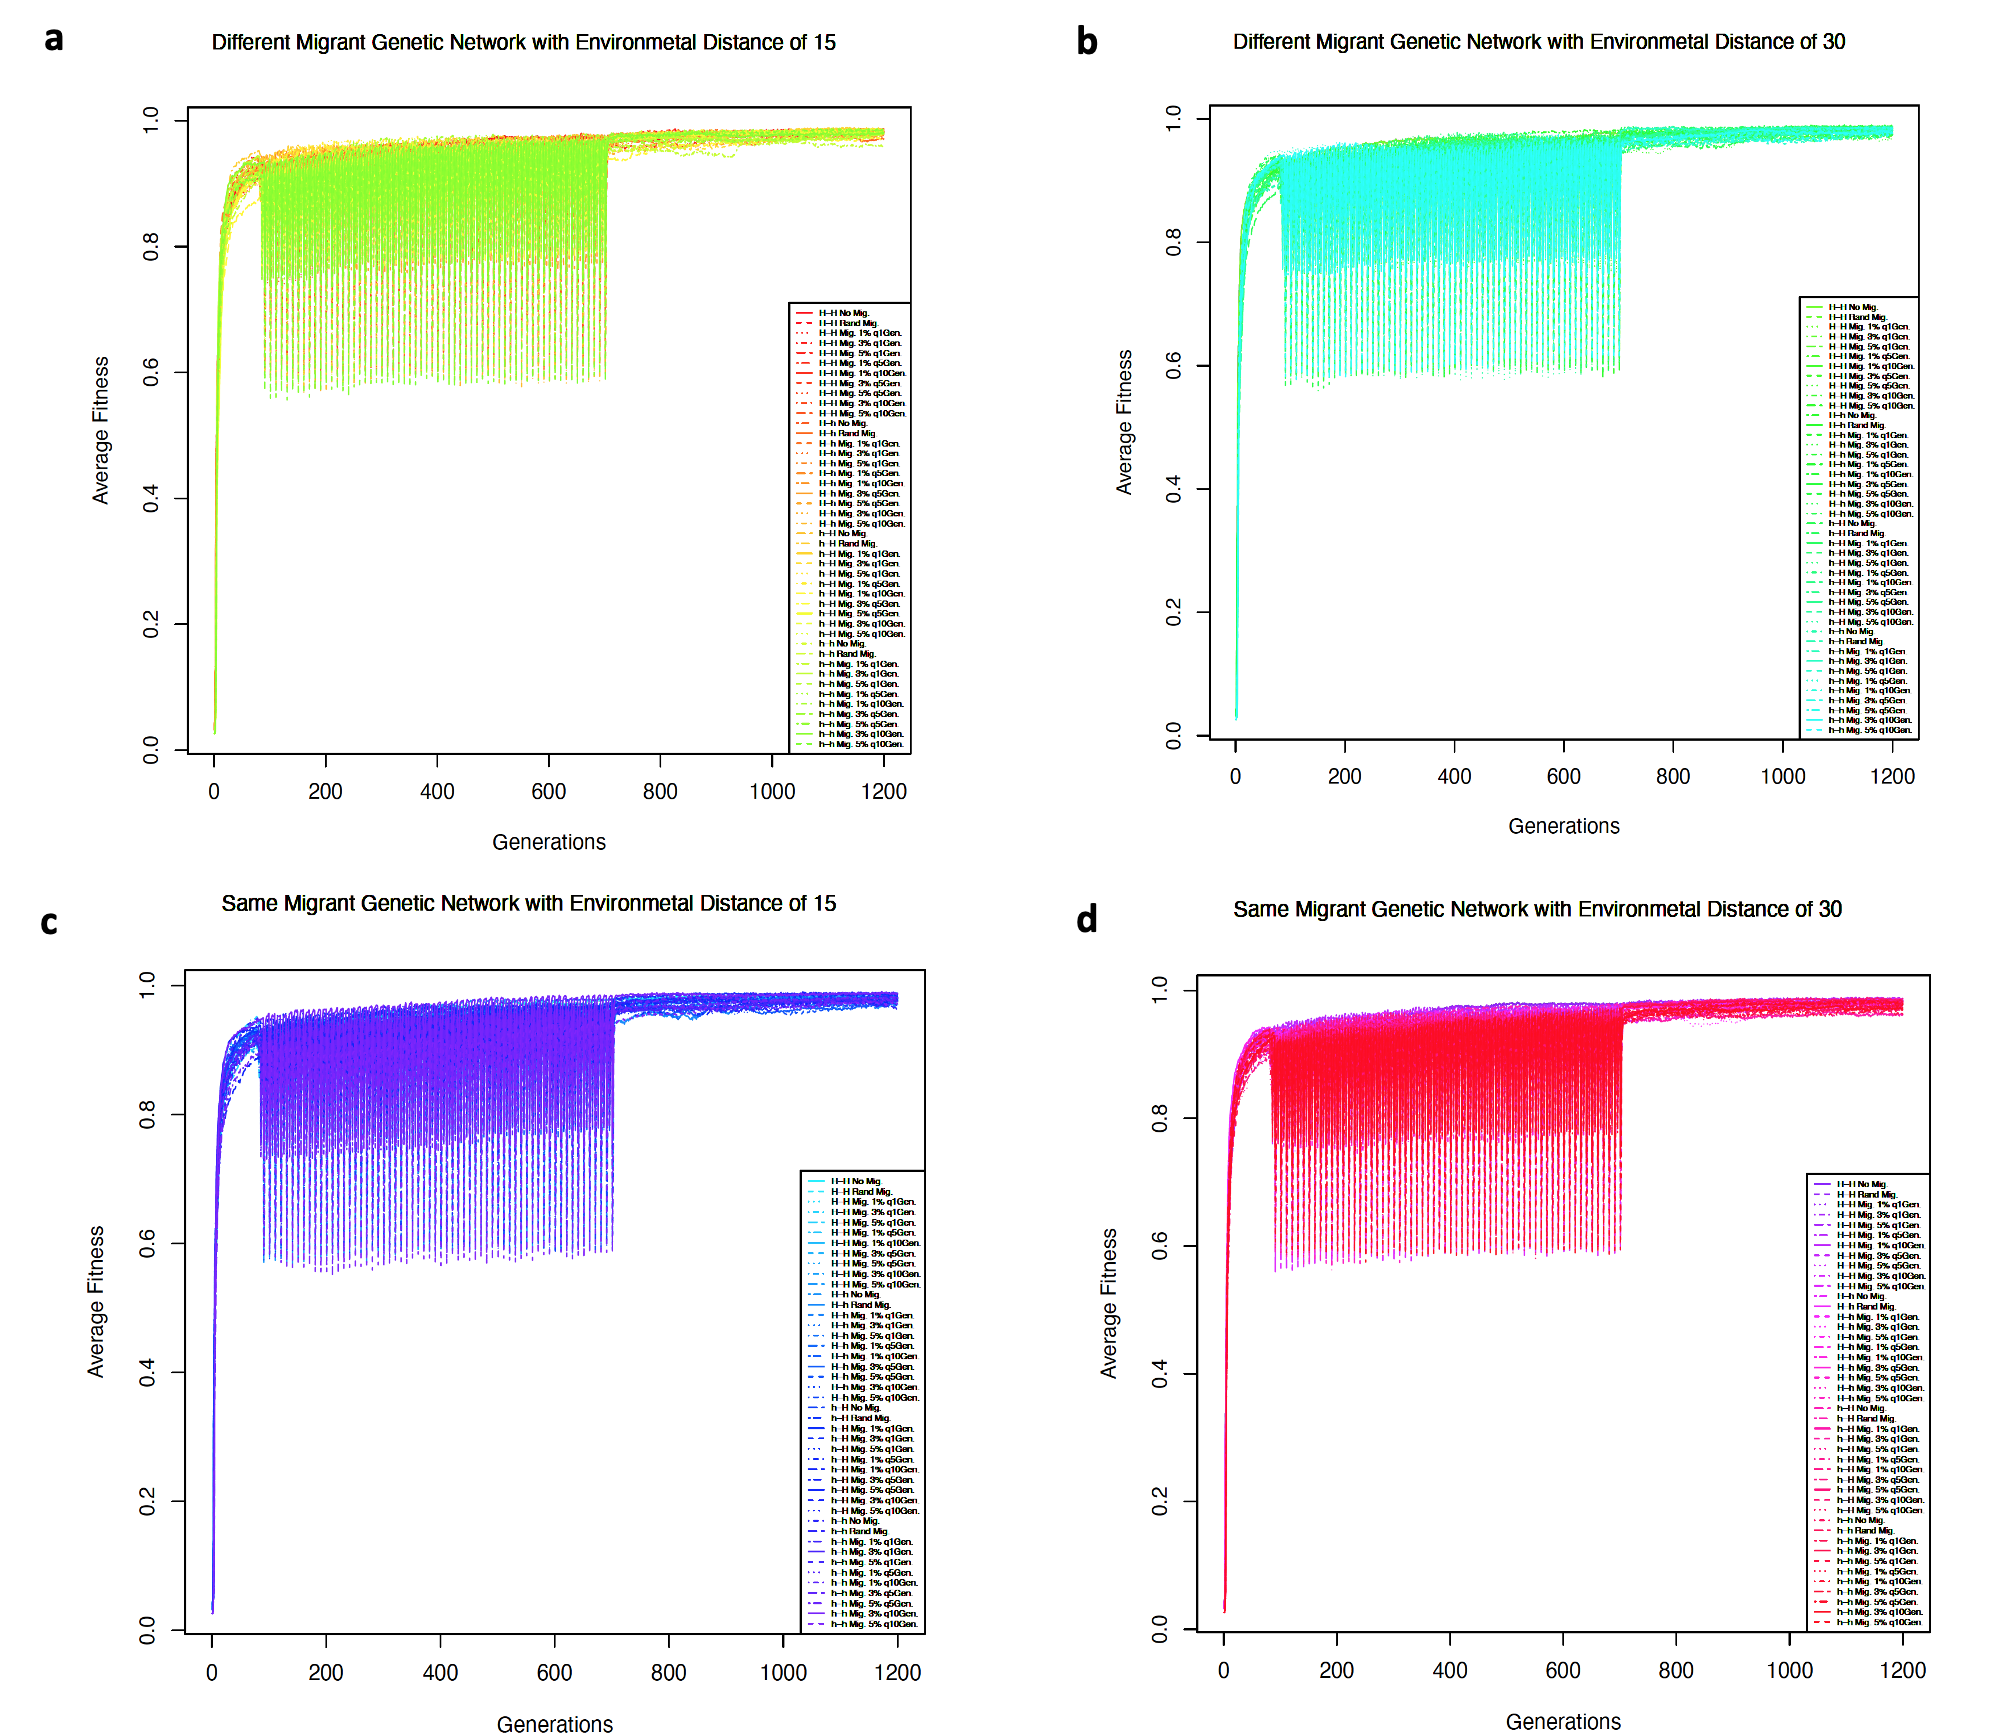
\includegraphics[scale=0.45]{../Results/migration.jpg}
    \caption{Plots showing the effect of migration on fitness over time. Migration occurs between generations 80 and 700, where the network gets 500 generations afterwards to try and recover. Each line is one of the 44 different starting conditions for the 4 combinations of genetic variant and environmental distance. ‘H’ means heterozygous while ‘h’ is homozygous, and ‘q’ means every. For example, ‘H-h Mig. 1\% q1Gen.’ is heterozygous (main population), homozygous (migrant population), migration rate of 1\% every generation. The graphs reveal the fluctuations in fitness values caused by gene flow where (a) shows the effect of migrant network with different regulations from the main population, evolving to a trait value of 65 (Environmental Distance of 15). It is a variation where gene $y_1$ negatively regulates gene $y_1$, and gene $y_2$ positively regulates the other genes, including gene $y_3$ which is the trait values. Mean fitness was 0.743, with a standard deviation of 0.375. (b) is a migrant network same as in graph (a) where the regulations are different, instead evolving to 80 (Environmental Distance of 30). Mean fitness value was 0.753, standard deviation of 0.364. (c) shows the effect of a migrant population but with the same regulations as in the main population. Therefore, gene $y_2$ is negatively regulated by gene $y_1$, and gene $y_1$ positively regulates the other genes. Similar to graph (a) it is evolving to a trait value of 65. Mean fitness of 0.769 and standard deviation of 0.359. (d) same regulation as the migrant network in graph (c) however evolves to a trait value of 80. Mean fitness of 0.743 and standard deviation of 0.381.}
    \label{fig:With Migration}
\end{figure}
\newpage
With migration, the genetic network was still able to evolve at time to high fitness value but there was greater variation. \textit{Figure 4} shows gene flow can disrupt the development of a genetic network. The average fitness for the different environmental distance and variant networks were lower compared to without migration. For a population that is starting as heterozygous, it evolves quickly at the start but gene flow causes large deviations away from the average fitness, dropping to almost half the average fitness. Constant fluctuations, dropping below 0.50 highlights how distant the trait values are in the Cauchy distribution. As mentioned before, it is a narrower distribution in the centre so deviations away from it can lower the fitness value by a significant amount.\\
\begin{wrapfigure}{l} {0.7\textwidth}
    \begin{center}
        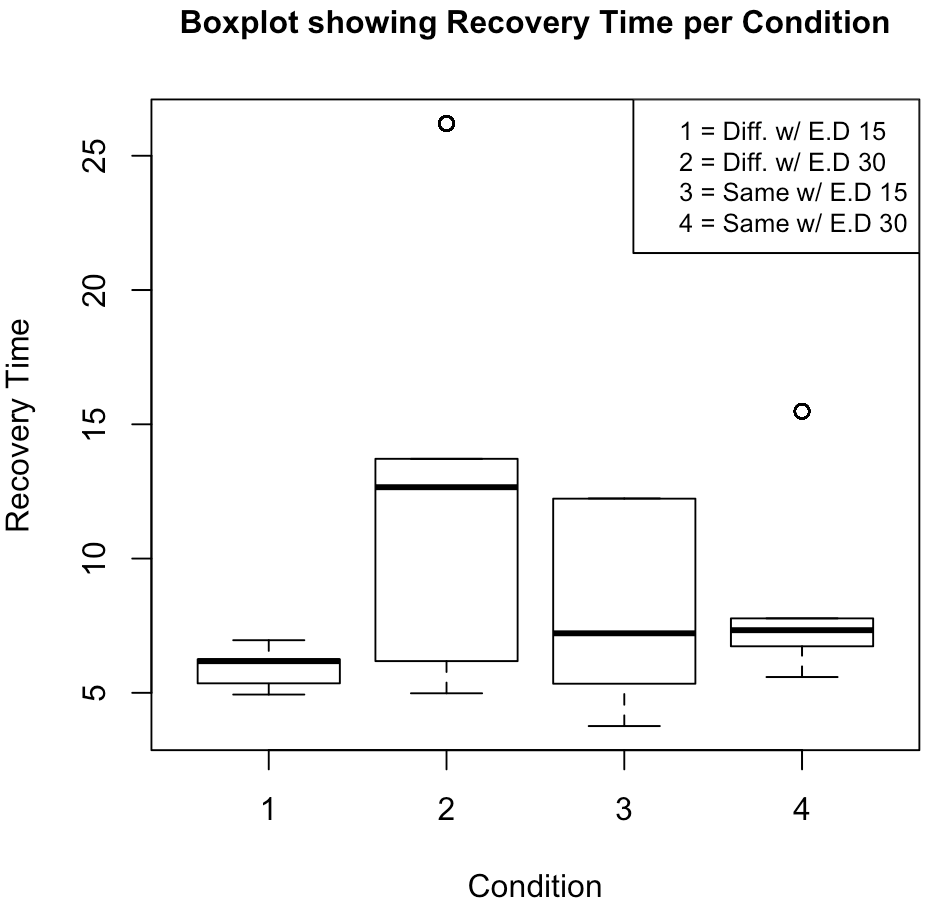
\includegraphics[scale=0.35]{../Results/boxplot_recovery_time.jpg}
    \end{center}
    \caption{Boxplot showing the recovery times of the two variant migrant genetic regulatory makeups, evolving to a trait value of 65 or 80. Two variants of the genetic regulation where one variant is the same as the main population, thus $gene_1$ positively regulates $gene_2$ and $gene_3$, and $gene_2$ negatively regulates $gene_1$, and the other variant is $gene_2$ positively regulating the other genes, while $gene_1$ negatively regulates $gene_2$. Average recovery time different variant evolving to a trait value of 65 is 5.94 generations (standard deviation 0.72 generations), and for the other evolving to 80, mean of 12.75 generations with standard deviation of 7.57 generations. For the same migrant regulatory network, recovery time average of 8.16 generations (standard deviation of 3.51 generations) for environmental distance of 15 and mean of 8.58 generations with standard deviation 3.54 generations for environmental distance 30.}
    \label{fig:Recovery time}
\end{wrapfigure}
After migration, the network shows the ability to recover and stabilise very quickly. Populations that evolved slowly at the start are likely populations starting with homozygous individuals. Rarely did the populations reached a fitness value of 1.00 however showed the ability to increase over time. The variation between the different genetic structures and environmental distances was quite high which is to be expected from the visualised deviations. As expected, average fitness is lower compared to without migration.\\
Although no statistical test was conducted to see effects of environmental distance and or genetic variant on recovery time, boxplot highlights the possibility alleles were able to persist longer, possible because they are beneficial, showing that developmental pattern could be context-dependent. The network recovery time for the different migrant regulatory network evolving to a trait value of 80 (environmental distance 30) did have the highest average of 12.75 generations but a standard deviation of 7.57, which could possibly be due to homogenous scenarios and slower evolution. For the same autoregulatory network motif, when the migrant population is evolving to a trait value of 15 (environmental distance of 65), it took an average of 8.16(standard deviation 3.51)  for the fitness value to equal or rise above the average fitness. The migrant network that evolved to trait value of 80 also showed consistent behaviours as it took a similar 8.58 generation recovery average, fluctuating between 3.54 generations.
\subsection{Robustness}
\begin{figure}[h!]
\centering
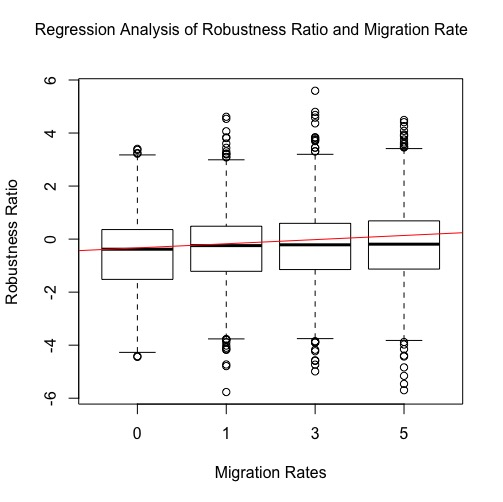
\includegraphics[scale=0.40]{../Results/robust_regression.jpg} \caption{Graph showing the plots of the regression analysis of the log of the variance ratio and migration pattern and genetic makeup of both populations. Analysis of variance results \textit{(see Appendix C)} show statistical significance of migration pattern on the log of the ratio. However, post hoc Tukey Tukey test \textit{(see Appendix C)} shows no statistical significance with a particular migration pattern and robustness ratio.} \label{fig: Regression}
\end{figure}
Multiple linear regression was done to see if any of the independent variables had a significant effect on the log robustness ratio. The data was log transformed to make it less skewed and linearise it. There were 4 factors: main population starting genetic makeup, migrant population starting genetic makeup, migration rate and migration pattern which were considered, as well as the interaction of starting genetic makeup of both populations (homozygous or heterozygous), and the interaction of migration rate and pattern. Migration rates were 1\%, 3\% and 5\%, while migration patterns were every generation, every 5 generations and every 10 generations. Analysis of variance result \textit{(see Appendix C)} reveals that the log ratio is statistically different for the migration patterns compared to the other factors. Linear regression computed an F-statistic of 3.25 with a corresponding p-values of 0.04, below the \textalpha level of 0.05. Before doing a post hoc Tukey test, Bartlett test was done to see homogeneity of variances (p-value of 0.32) and normal quantile plots created to see if data distribution was relatively normal \textit{(see Appendix C)}. Ends of the normal QQ-plot deviated a bit suggesting a symmetric distribution that is fat-tailed. This is to be expected as due to the range of values present when migration is occurring. Post hoc Tukey analysis \textit{(see Appendix C)} revealed no significant effect of any particular migration pattern however that could be due to small sample sizes.
